% Supported aspectratio 43|169, default is 43
\documentclass[aspectratio=169]{beamer}
\usetheme[theme=blue,logo=logowithtextvi]{HUST} % <-- this matches beamerthemeHUST.sty

% \usepackage[utf8]{vietnam}
\usepackage[T5]{fontenc}
\usepackage{lmodern}
% \setmainfont{assets/fonts/LATO-BLACK.TTF}
\usepackage{enumitem}
\usepackage{tcolorbox}
\usepackage{listings}
\usepackage{verbatim}
\usepackage{amsmath}
\usepackage[table]{xcolor}
\usepackage{tikz}
\usepackage{minted}

\usetikzlibrary{decorations.pathreplacing,arrows.meta}

\tcbuselibrary{listingsutf8}




\newcommand{\placecontent}[4]{%
  \tikz[remember picture,overlay]
    \node[anchor=north west]
      at ([xshift=#1,yshift=-#2]current page.north west)
      {\parbox{#3}{#4}};
}


\title{CẤU TRÚC DỮ LIỆU VÀ THUẬT TOÁN}
\author{SoICT - HUST}
\date{}
\setbeamertemplate{footline}{%
  \hfill%
  \insertframenumber\hspace{0.5cm}\vspace{0.3cm}
  }
\begin{document}

\HUSTInsertBrandSlide
\HUSTInsertThemeSlide

% Title slide - place it here for your customization
{\HUSTUseBackground{onelove.pdf}
\begin{frame}
  \ifdefstring{\insertaspectratio}{169}{
    \HUSTCornerImage{assets/logo/04.pdf}

    %----------You can edit here----------
    \placecontent{0.5cm}{0.33\paperheight}{0.85\paperwidth}{
        \color{\HUSTFrameTitleTextColor}\bfseries\fontsize{22pt}{30pt}\selectfont
        \inserttitle
    }
    % \placecontent{0.5cm}{0.48\paperheight}{10cm}{    % one-line title
    \placecontent{0.5cm}{0.60\paperheight}{0.5\paperwidth}{    % two-line title
        \color{\HUSTFrameTitleTextColor}\fontsize{12pt}{14pt}\selectfont
        TUẦN 1 : CÁC KHÁI NIỆM CƠ BẢN\\
        \insertauthor
    }
  }{}
  \ifdefstring{\insertaspectratio}{43}{
    \HUSTCornerImage[0.1][0.35cm][-0.03]{assets/logo/04.pdf}

    %----------You can edit here----------
    \placecontent{0.5cm}{0.33\paperheight}{0.80\paperwidth}{
        \color{\HUSTFrameTitleTextColor}\bfseries\fontsize{18pt}{22pt}\selectfont
        \inserttitle
    }
    % \placecontent{0.5cm}{0.48\paperheight}{10cm}{    % one-line title
    \placecontent{0.5cm}{0.60\paperheight}{0.5\paperwidth}{    % two-line title
        \color{\HUSTFrameTitleTextColor}\fontsize{12pt}{14pt}\selectfont
        TUẦN 1 : CÁC KHÁI NIỆM CƠ BẢN\\
        \insertauthor
    }
  }{}
\end{frame}
}

% Display the tableofcontents before a section
\AtBeginSection[]
{
    \begin{frame}<beamer>
        \frametitle{MỤC LỤC}
        \tableofcontents[currentsection]
    \end{frame}
}

%Phần này không cần chỉnh theo tỉ lệ slide 43 69 "
\begin{frame}{MỤC TIÊU}
    \hspace{1.5cm}\textit{\color{HUSTBlue}Sau bài học này, người học có thể:}\vspace{0.5cm}

    \begin{itemize}
        \item 1. Hiểu được một số \textcolor{HUSTRed}{khái niệm cơ bản về thuật toán}
        \item 2. Biết \textcolor{HUSTRed}{ký hiệu tiệm cận} dùng để đánh giá độ phức tạp thuật toán
        \item 3. Biết cách \textcolor{HUSTRed}{phân tích độ phức tạp của thuật toán}
    \end{itemize}
  
\end{frame}

%slide 1 section 1
\section{Ví dụ minh họa}
\begin{frame}{1. Ví dụ minh họa}
  \begin{itemize}[label={\tiny$\blacksquare$}] 
    \item {\color{HUSTBlue}Bài toán tìm dãy con lớn nhất:}
      \begin{itemize}[label={\tiny$\bullet$}]
        \item Cho dãy số gồm $n$ số: $a_0, a_1, a_2, ..., a_{n-1}$

        \item Dãy gồm liên tiếp các số $a_i, a_{i+1},\ldots,a_j$ với $0 \leq i \leq j \leq n-1$ được gọi là 
          \textcolor{HUSTYellow}{dãy con} của dãy đã cho và $\sum_{k=i}^j a_k$ được gọi là trọng lượng của dãy con này
        \item \color{HUSTYellow}\textbf{Hãy tìm trọng lượng lớn nhất của dãy con, tức là tìm cực đại giá trị} $\sum_{k=i}^j a_k$ . Ta gọi dãy con có trọng lượng lớn nhất là \textbf{dãy con lớn nhất.}
    \end{itemize}
    \pause
  \item \textbf{Ví dụ:} Cho dãy số $-2, \textcolor{HUSTYellow}{11, -4, 13}, -5, 2$ thì cần đưa ra câu trả lời là 20 (dãy con lớn nhất là 11, -4, 13 với giá trị $= 11 + (-4) + 13 = 20$)
\end{itemize}

\end{frame}
% "

%slide 2 section 1

\begin{frame}[fragile]{1. Ví dụ minh họa}
  \begin{itemize}[label={\tiny$\blacksquare$}]
    \item {\color{HUSTBlue}Cách 1: Duyệt toàn bộ}
      \begin{itemize}[label={\tiny$\bullet$}]
        \item Duyệt tất cả các dãy con có thể có của dãy đã cho:
          \textcolor{HUSTYellow}{$a_i, a_{i+1},\ldots,a_j$ với $0 \leq i \leq j \leq n-1$,}
          và tính tổng của mỗi dãy con để tìm ra trọng lượng lớn nhất.
      \end{itemize}
  \end{itemize}
% code C in box


\vspace{0.5em}

\begin{center}
\begin{tcolorbox}[colback=gray!10, colframe=black,boxrule=0.6pt,
    width=0.5\textwidth]
\scriptsize
\begin{lstlisting}[language=C, basicstyle=\ttfamily\tiny\color{HUSTYellow}, breaklines=true]
int maxSum = a[0];
for (int i = 0; i <= n-1; i++) {
    for (int j = i; j <= n-1; j++) {
        int sum = 0;
        for (int k = i; k <= j; k++)
            sum += a[k];
        if (sum > maxSum) maxSum = sum;
    }
}
\end{lstlisting}
\end{tcolorbox}
\end{center}
\end{frame}


%slide 3 section 1
\begin{frame}[fragile]{1. Ví dụ minh họa}
\begin{itemize}
    \item Cách 1: Duyệt toàn bộ
    \begin{itemize}
        \item Duyệt tất cả các dãy con có thể có của dãy đã cho: $a_i, a_{i+1}, ..., a_j$ với $0 \leq i \leq j \leq n-1$, và tính tổng của mỗi dãy con để tìm ra trọng lượng lớn nhất.
        \item \textbf{Phân tích thuật toán:} Ta sẽ tính số lượng phép cộng mà thuật toán phải thực hiện, tức là đếm xem dòng lệnh \texttt{\textcolor{HUSTYellow}{sum += a[k]}} phải thực hiện bao nhiêu lần. Số lượng phép cộng là:
    \end{itemize}
\end{itemize}

%columns

\begin{columns}[T,onlytextwidth]
    \begin{column}{0.45\textwidth}
        \begin{tcolorbox}[colback=gray!10, colframe=black, boxsep=0.1pt, left=0.1pt, right=0.1pt, top=0.1pt, bottom=0.1pt]
            \tiny
\begin{lstlisting}[language=C, basicstyle=\ttfamily\tiny\color{HUSTBlue}, breaklines=true,escapeinside={(*@}{@*)} ]
int maxSum = a[0];
for (int i = 0; i<=n-1; i++) {
  for (int j = i; j<=n-1; j++) {
    int sum = 0;
    for (int k=i; k<=j; k++) (*@\textcolor{HUSTRed}{sum += a[k];}@*)
    if (sum > maxSum) maxSum = sum;
  }
}
\end{lstlisting}
        \end{tcolorbox}
    \end{column}

\hspace{0.5em}
    \begin{column}{0.55\textwidth}
        \tiny\color{HUSTBlue}
        \begin{align*}
    &\sum_{i=0}^{n-1} \sum_{j=i}^{n-1} (j-i+1)
    = \sum_{i=0}^{n-1} \left( 1 + 2 + \cdots + (n-i) \right)
    = \sum_{i=0}^{n-1} \frac{(n-i)(n-i+1)}{2} \\
    &= \frac{1}{2} \sum_{k=1}^n k(k+1)
    = \frac{1}{2} \left[ \sum_{k=1}^n k^2 + \sum_{k=1}^n k \right] 
    = \frac{1}{2} \left[ \frac{n(n+1)(2n+1)}{6} + \frac{n(n+1)}{2} \right] \\
    &= \frac{n^3}{6} + \frac{n^2}{2} + \frac{n}{3}
\end{align*}
    \end{column}

\end{columns}
\end{frame}

%slide 4 section 1
\begin{frame}{1. Ví dụ minh họa}
  \begin{itemize}[label={\tiny$\blacksquare$}]
    \item {\color{HUSTBlue}Cách 2: Duyệt toàn bộ có cải tiến:}
    
    \begin{center}
    \renewcommand{\arraystretch}{1.3}
    \begin{tabular}{>{\raggedright\arraybackslash}p{1.6cm} 
                    >{\centering\arraybackslash}p{1cm} 
                    >{\centering\arraybackslash}p{1cm} 
                    >{\centering\arraybackslash}p{1cm} 
                    >{\centering\arraybackslash}p{1cm} 
                    >{\centering\arraybackslash}p{1cm} 
                    >{\centering\arraybackslash}p{1cm}}
         \rowcolor{orange!80}
        \textcolor{white}{Index i} & \textcolor{white}{0} & \textcolor{white}{1} & \textcolor{white}{2} & \textcolor{white}{3} & \textcolor{white}{4} & \textcolor{white}{5} \\
         \rowcolor{orange!15}
        a[i] & -2 & 11 & -4 & 13 & -5 & 2 \\
    \end{tabular}
    \end{center}

    \textcolor{orange!80!black}{$i = 0$:}

\centering
\scriptsize

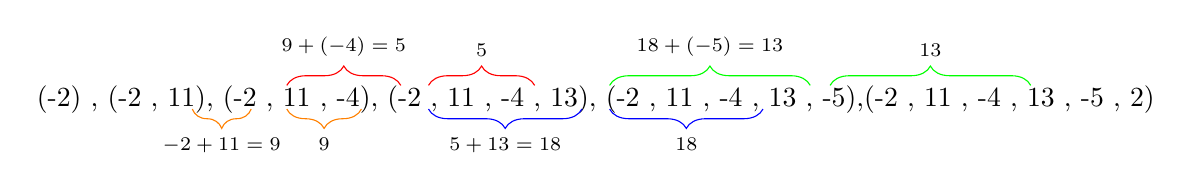
\begin{tikzpicture}[baseline]
    \node (A) at (0,0) {(-2) , (-2 , 11), (-2 , 11 , -4), (-2 , 11 , -4 , 13), (-2 , 11 , -4 , 13 , -5),(-2 , 11 , -4 , 13 , -5 , 2)};
 
    \node (X1) at (-5,0) {};
    \node (X2) at (-4.5,0) {};
    \node (X3) at (-3.8,0) {};
    \node (X4) at (-3.1,0) {};
    \node (Y1) at (-3.8,0.3) {};
    \node (Y2) at (-2.6,0.3) {};
    \node (Y3) at (-2,0.3) {};
    \node (Y4) at (-0.9,0.3) {};
    \node (Z1) at (-2,0) {};
    \node (Z2) at (-0.3,0) {};
    \node (Z3) at (0.3,0) {};
    \node (Z4) at (2,0) {};
    \node (A1) at (0.3,0.3) {};
    \node (A2) at (2.6,0.3) {};
    \node (A3) at (3.1,0.3) {};
    \node (A4) at (5.4,0.3) {};

    \draw [decorate, decoration={brace,amplitude=7pt,mirror}, orange]
        (X1.south west) -- (X2.south east) node[midway, below=7pt, black] {\scriptsize $-2+11 = 9$};
    \draw [decorate, decoration={brace,amplitude=7pt,mirror}, orange]
        (X3.south west) -- (X4.south east) node[midway, below=7pt, black] {\scriptsize $9$};
    \draw [decorate, decoration={brace,amplitude=7pt}, red]
        (Y1.south west) -- (Y2.south east) node[midway, above=7pt, black] {\scriptsize $9+(-4)=5$};
    \draw [decorate, decoration={brace,amplitude=7pt}, red]
        (Y3.south west) -- (Y4.south east) node[midway, above=7pt, black] {\scriptsize $5$};
    \draw [decorate, decoration={brace,amplitude=7pt,mirror}, blue]
        (Z1.south west) -- (Z2.south east) node[midway, below=7pt, black] {\scriptsize $5+13 = 18$};
    \draw [decorate, decoration={brace,amplitude=7pt,mirror}, blue]
        (Z3.south west) -- (Z4.south east) node[midway, below=7pt, black] {\scriptsize $18$};
    \draw [decorate, decoration={brace,amplitude=7pt}, green]
        (A1.south west) -- (A2.south east) node[midway, above=7pt, black] {\scriptsize $18+(-5)=13$};
    \draw [decorate, decoration={brace,amplitude=7pt}, green]
        (A3.south west) -- (A4.south east) node[midway, above=7pt, black] {\scriptsize $13$};

\end{tikzpicture}

\vspace{0.5em}

      \begin{itemize}[label={\tiny$\bullet$}]
        \item Nhận thấy, ta có thể tính tổng các phần tử từ vị trí $i$ đến $j$ từ tổng của các phần tử từ $i$ đến $j-1$ chỉ bằng 1 phép cộng:
      \end{itemize}

\vspace{-4em}

\color{HUSTRed}\large
        \[
        \sum_{k=i}^j a[k] = a[j] + \sum_{k=i}^{j-1} a[k]
        \]
  \begin{center}
    \vspace{-1em}
    \begin{tikzpicture}
    \node (X1) at (-4,0) {};
    \node (X2) at (-3,0) {};
    \node (X3) at (-1,0) {};
    \node (X4) at (-0,0) {};
        
    \draw [decorate, decoration={brace,amplitude=7pt,mirror}, blue]
        (X1.north west) -- (X2.north east) node[midway, below=7pt, black,xshift=-40pt] {\scriptsize Tổng các phần tử từ i đến j};
    \draw [decorate, decoration={brace,amplitude=7pt,mirror}, blue]
        (X3.north west) -- (X4.north east) node[midway, below=7pt, black,xshift=40pt] {\scriptsize Tổng các phần tử từ i đến j-1};
    \end{tikzpicture}
  \end{center}
\end{itemize}
\end{frame}

%slide 5 section 1
\begin{frame}[fragile]{1. Ví dụ minh họa}
  \color{HUSTRed}\large
        \[
        \sum_{k=i}^j a[k] = a[j] + \sum_{k=i}^{j-1} a[k]
        \]
  \begin{center}
    \begin{tikzpicture}
    \node (X1) at (-4,0) {};
    \node (X2) at (-3,0) {};
    \node (X3) at (-1,0) {};
    \node (X4) at (-0,0) {};
        
    \draw [decorate, decoration={brace,amplitude=7pt,mirror}, blue]
        (X1.north west) -- (X2.north east) node[midway, below=7pt, black,xshift=-40pt] {\scriptsize Tổng các phần tử từ i đến j};
    \draw [decorate, decoration={brace,amplitude=7pt,mirror}, blue]
        (X3.north west) -- (X4.north east) node[midway, below=7pt, black,xshift=40pt] {\scriptsize Tổng các phần tử từ i đến j-1};
    \end{tikzpicture}
  \end{center}
\vspace{-1em}
\begin{center}
\begin{tikzpicture}
  \node[inner sep=0pt] (box1) at (0,0) {
  % Node đầu là bảng code 1
    %C code1
    \begin{minipage}{0.42\textwidth}
        \begin{tcolorbox}[colback=gray!10, colframe=black, boxsep=0.1pt, left=0.1pt, right=0.1pt, top=0.1pt, bottom=0.1pt]
            \tiny
\begin{lstlisting}[language=C, basicstyle=\ttfamily\tiny\color{HUSTBlue}, breaklines=true ]
int maxSum = a[0];
for (int i=0; i<=n-1; i++) {
  for (int j=i; j<=n-1; j++) {
    int sum = 0;
    for (int k=i; k<=j; k++) sum += a[k];
    if (sum > maxSum) maxSum = sum;
  }
}
        \end{lstlisting}
      \end{tcolorbox}
    \end{minipage}
};

    %C code 2
    \node[inner sep=0pt] (box2) at (6.5,0) {
    \begin{minipage}{0.4\textwidth}
        \begin{tcolorbox}[colback=gray!10, colframe=black, boxsep=0.1pt, left=0.1pt, right=0.1pt, top=0.1pt, bottom=0.1pt]
            \tiny
\begin{lstlisting}[language=C, basicstyle=\ttfamily\tiny\color{HUSTBlue}, breaklines=true]
int maxSum = a[0];
for (int i=0; i<=n-1; i++) {
  int sum = 0;
  for (int j=i; j<=n-1; j++) {
    sum += a[j];
    if (sum > maxSum) maxSum = sum;
  }
}
        \end{lstlisting}
      \end{tcolorbox}
\end{minipage}
};
  \draw[line width=3mm ,-{Latex[length=8pt, width=14pt]}, orange] 
    ([xshift=0.05cm]box1.east)-- ([xshift=-0.05cm]box2.west);
\end{tikzpicture}
\end{center}
\end{frame}

%slide 6 section 1
\begin{frame}[fragile]{1. Ví dụ minh họa}
\begin{itemize}[label={\tiny$\blacksquare$}] 
    \item {\color{HUSTBlue}Cách 2: duyệt toàn bộ có cải tiến}
      \begin{itemize}[label={\tiny$\bullet$}]
        \item Phân tích thuật toán: Ta sẽ tính số lượng phép cộng mà thuật toán phải thực hiện, tức là
đếm xem dòng lệnh \textcolor{HUSTRed}{sum += a[j]} phải thực hiện bao nhiều lần. Số lượng
phép cộng là:
    \end{itemize}
  \end{itemize}
\color{HUSTRed}\large
        \[
         \sum_{i=0}^{n-1} (n-i) = n + (n-1) + \ldots + 1 = \frac{n^{2}}{2} + \frac{n}{2}
        \]
\begin{center}
\begin{tcolorbox}[colback=gray!10, colframe=black,boxrule=0.6pt,
    width=0.5\textwidth]
\tiny
\begin{lstlisting}[language=C, basicstyle=\ttfamily\tiny\color{HUSTBlue}, breaklines=true]
int maxSum = a[0];
for (int i=0; i<=n-1; i++) {
  int sum = 0;
    for (int j=i; j<=n-1; j++) {
      sum += a[j];
      if (sum > maxSum) maxSum = sum;
    }
}
\end{lstlisting}
\end{tcolorbox}
\end{center}
\end{frame}

%slide 7 section 1
\begin{frame}[fragile]{1. Ví dụ minh họa}
\begin{itemize}[label={\tiny$\blacksquare$}] 
    \item Số lượng phép cộng mà mỗi thuật toán cần thực hiện là:
      \begin{itemize}[label={\tiny$\bullet$}]
        \item Cách 1. Duyệt toàn bộ \hspace{0.5cm}\textcolor{HUSTRed}{\large$\displaystyle\frac{n^{3}}{6} + \frac{n^{2}}{2} + \frac{n}{3}$}
        \item Cách 2. Duyệt toàn bộ có cải tiến \hspace{0.5cm}\textcolor{HUSTRed}{\large$\displaystyle\frac{n^{2}}{2} + \frac{n}{2}$}
      \end{itemize}
    \item Cùng một bài toán, ta đã đề xuất 2 thuật toán đòi hỏi số lượng phép toán khác nhau, và vì thế
sẽ đòi hỏi thời gian tính khác nhau.
    \item Bảng dưới đây cho thấy thời gian tính của 2 thuật toán trên, với giả thiết: máy tính có thể
thực hiện $10^{8}$ phép cộng trong một giây
  \end{itemize}

%board
\vspace{0.1cm}

\begin{center}
\tiny
\renewcommand{\arraystretch}{1.4}
\begin{tabular}{
  |>{\centering\arraybackslash}m{1.3cm}
  |>{\columncolor{gray!15}\centering\arraybackslash}m{0.8cm}
  |>{\columncolor{gray!15}\centering\arraybackslash}m{1.1cm}
  |>{\columncolor{gray!15}\centering\arraybackslash}m{0.8cm}
  |>{\columncolor{gray!15}\centering\arraybackslash}m{1.1cm}
  |>{\columncolor{HUSTYellow}\centering\arraybackslash}m{0.8cm}
  |>{\columncolor{HUSTYellow}\centering\arraybackslash}m{1.1cm}
  |>{\columncolor{HUSTYellow}\centering\arraybackslash}m{0.8cm}
  |>{\columncolor{HUSTYellow}\centering\arraybackslash}m{1.1cm}|}
\hline
\textbf{Độ phức tạp} & \textbf{$n=10$} & \textbf{Thời gian} & \textbf{$n=100$} & \textbf{Thời gian} & \textbf{$n=10^{4}$} & \textbf{Thời gian} & \textbf{$n=10^{6}$} & \textbf{Thời gian} \\
\hline
\textbf{$n^{3}$} & $10^{3}$ & $10^{-5}$ giây & $10^{6}$ & $10^{-2}$ giây & $10^{12}$ & 2.7 giờ & $10^{18}$ & 115 ngày \\
\hline
\textbf{$n^{2}$} & $100$ & $10^{-6}$ giây & $10\,000$ & $10^{-4}$ giây & $10^{8}$ & 1 giây & $10^{12}$ & 2.7 giờ \\
\hline
\end{tabular}
\end{center}


\end{frame}

%slide 1 section 2
\section{Một số khái niệm cơ bản về thuật toán}
\begin{frame}{2. Một số khái niệm cơ bản về thuật toán}
\begin{itemize}[label={\tiny$\blacksquare$}] 
    \item Thuật toán (Algorithm) giải bài toán đặt ra là một thủ tục xác định bao gồm \textcolor{HUSTRed}{một dãy hữu
hạn các bước cần thực hiện} để \textbf{thu được đầu ra (output) từ một đầu vào cho trước
(input)} của bài toán.

%cần nhét ảnh gốc vào

    \item Một số đặc trưng cơ bản của thuật toán:
      \begin{itemize}[label={\tiny$\bullet$}]
        \item Chính xác
        \item Hữu hạn
        \item Đơn trị
        \item Tổng quát
      \end{itemize}
  \end{itemize}
\end{frame}

%slide 2 section 2
\begin{frame}{2. Một số khái niệm cơ bản về thuật toán}
\begin{itemize}[label={\tiny$\blacksquare$}] 
    \item {\color{HUSTBlue}Độ phức tạp của thuật toán:}
    
    \begin{itemize}[label={\tiny$\bullet$}]
        \item {\color{HUSTBlue}Khi nói đến hiệu quả của một thuật toán, ta quan tâm đến chi phí cần dùng để thực hiện nó:}
        
        \vspace{0.3cm}
        \begin{itemize}
            \item {\color{HUSTBlue}1) Dễ hiểu, dễ cài đặt, dễ sửa đổi ?}
            
            \item {\color{HUSTBlue}2) Thời gian sử dụng CPU ? \textcolor{HUSTRed}{\textbf{THỜI GIAN}}}
            
            \item {\color{HUSTBlue}3) Tài nguyên bộ nhớ ? \textcolor{HUSTRed}{\textbf{BỘ NHỚ}}}
        \end{itemize}
        
    \end{itemize}
    
\end{itemize}
\end{frame}

%slide 3 section 2
\begin{frame}[plain]{2. MỘT SỐ KHÁI NIỆM CƠ BẢN VỀ THUẬT TOÁN}
\hspace*{-1cm}
\color{HUSTBlue}
\begin{minipage}{1.1\textwidth}
\begin{itemize}
    \item[{\tiny$\blacksquare$}] Độ phức tạp của thuật toán:
    
    \begin{itemize}
        \item[{$\bullet$}] Làm thế nào để đo được thời gian tính?
        
        \begin{itemize}
            \item[{\fontsize{4}{5}\selectfont$\blacksquare$}] Thời gian tính của thuật toán phụ thuộc vào dữ liệu vào (kích thước tăng, thì thời gian tăng).
            \vspace{0.2cm}
            \item[{\fontsize{4}{5}\selectfont$\blacksquare$}] Vì vậy, người ta tìm cách đánh giá thời gian tính của thuật toán bởi một hàm của độ dài dữ liệu đầu vào. Tuy nhiên, trong một số trường hợp, kích thước dữ liệu đầu vào là như nhau, nhưng thời gian tính lại rất khác nhau.
            
            \begin{itemize}
                \item[$\bullet$] Ví dụ: Để tìm số nguyên tố đầu tiên có trong dãy: ta duyệt dãy từ trái sang phải
                
                \vspace{0.2cm}
                Dãy 1: 3 \; 9 \; 8 \; 12 \; 15 \; 20 \; (thuật toán dừng ngay khi xét phần tử đầu tiên)
                
                Dãy 2: 9 \; 8 \; 3 \; 12 \; 15 \; 20 \; (thuật toán dừng khi xét phần tử thứ ba)
                
                Dãy 3: 9 \; 8 \; 12 \; 15 \; 20 \; 3 \; (thuật toán dừng khi xét phần tử cuối cùng)
                
                \vspace{0.2cm}
                $\rightarrow$ 3 loại thời gian tính
                
            \end{itemize}
        \end{itemize}
        
    \end{itemize}
    
\end{itemize}
\end{minipage}
\end{frame}

%slide 4 section 2
\begin{frame}[t]{2. MỘT SỐ KHÁI NIỆM CƠ BẢN VỀ THUẬT TOÁN}

\begin{itemize}
    \item[\tiny$\blacksquare$] Các loại thời gian tính của thuật toán:
    
    \begin{itemize}
        \item[\tiny$\bullet$] \textcolor{HUSTBlue}{\textbf{Thời gian tính tốt nhất (Best-case)}}
    \end{itemize}
    
    \vspace{0.2cm}

    T($n$): thời gian tối thiểu cần thiết để thực hiện thuật toán với mọi bộ dữ liệu đầu vào kích thước $n$.
    
    \vspace{0.3cm}
    
    \begin{itemize}
        \item[\tiny$\bullet$] \textcolor{HUSTBlue}{\textbf{Thời gian tính trung bình (Average-case)}}
    \end{itemize}
    
    \vspace{0.2cm}
    T($n$): thời gian trung bình cần thiết để thực hiện thuật toán trên tập hữu hạn các đầu vào kích thước $n$.
    
    \vspace{0.3cm}
    
    \begin{itemize}
        \item[\tiny$\bullet$] \textcolor{HUSTBlue}{\textbf{Thời gian tính tồi nhất (Worst-case)}}
    \end{itemize}
    
    \vspace{0.2cm}
    T($n$): thời gian nhiều nhất cần thiết để thực hiện thuật toán với mọi bộ dữ liệu đầu vào kích thước $n$.
    
\end{itemize}

\end{frame}

%slide 5 section 2

\begin{frame}[fragile]{2. MỘT SỐ KHÁI NIỆM CƠ BẢN VỀ THUẬT TOÁN}

\begin{itemize}
    \item[\tiny$\blacksquare$] Có hai cách để đánh giá thời gian tính:
    \begin{itemize}
        \item[$\bullet$] \textbf{\textcolor{HUSTBlue}{Từ thời gian chạy thực nghiệm:}}
            \begin{itemize}
                \item[\tiny$\bullet$] cài đặt thuật toán, rồi chọn các bộ dữ liệu đầu vào thử nghiệm
                \item[\tiny$\bullet$] chạy chương trình với các dữ liệu đầu vào kích thước khác nhau
                \item[\tiny$\bullet$] sử dụng hàm \texttt{\textcolor{HUSTBlue}{clock()}} để đo thời gian chạy chương trình
            \end{itemize}
            \vspace{0.1cm}
            % Mã code C:
            \begin{center}
            
            \begin{tcolorbox}[colback=gray!10, colframe=black,boxrule=0.6pt,
    width=0.7\textwidth]
            \tiny
                \begin{lstlisting}[language=C, basicstyle=\ttfamily\tiny\color{HUSTBlue}, breaklines=true]
clock_t startTime = clock();
doSomeOperation();
clock_t endTime = clock();
clock_t clockTicksTaken = endTime - startTime;
double timeInSeconds = clockTicksTaken / (double) CLOCKS_PER_SEC;
                \end{lstlisting}
            \end{tcolorbox}
          \end{center}
        \item[$\bullet$] \textbf{\textcolor{HUSTBlue}{Lý thuyết: khái niệm xấp xỉ tiệm cận}}
    \end{itemize}
\end{itemize}
\end{frame}

%slide 1 section 3
\section{Ký hiệu tiệm cận}
\begin{frame}{3. Ký hiệu tiệm cận}
\begin{itemize}
    \item[\tiny$\blacksquare$] Các ký hiệu tiệm cận (\textit{asymptotic notation}):
    
    \vspace{0.2cm}
    
    \begin{center}
        {\Large
            \textcolor{HUSTRed}{$\Theta,\, \Omega,\, O,\, \omega$}
        }
    \end{center}
    
    \vspace{0.2cm}
    
    \begin{itemize}
        \item[\tiny$\bullet$] \textcolor{HUSTBlue}{Được sử dụng để mô tả thời gian tính của thuật toán, mô tả tốc độ tăng của thời gian chạy phụ thuộc vào kích thước dữ liệu đầu vào.}
        
        \vspace{0.2cm}
        
        \item[\tiny$\bullet$] \textcolor{HUSTBlue}{Ví dụ, khi nói thời gian tính của thuật toán cỡ $\Theta(n^2)$, tức là, thời gian tính tỉ lệ thuận với $n^2$ cộng thêm các đa thức bậc thấp hơn.}
    \end{itemize}
\end{itemize}
\end{frame}

%slide 2 section 3
\begin{frame}{3. Ký hiệu tiệm cận}
\textbf{3.1. Ký hiệu tiệm cận theta \textcolor{HUSTBlue}{$\Theta$}}
    
    \begin{itemize}

        \item[\tiny$\blacksquare$] Đối với hàm $g(n)$ cho trước, ta ký hiệu $\Theta(g(n))$ là tập các hàm:

% Định nghĩa Theta
\begin{center}
\begin{minipage}{0.9\textwidth}

\begin{center}

  \color{HUSTRed}

$\Theta(g(n)) = \{f(n):$ tồn tại các hằng số $c_1, c_2$ và $n_0$ sao cho:\\
  \vspace{0.2cm}
$0 \leq c_1g(n) \leq f(n) \leq c_2g(n)$, với mọi $n \geq n_0\}$\\
  \vspace{0.2cm}
 
  \color{black}
(tập tất cả các hàm có cùng tốc độ tăng với hàm $g(n)$)\\

\end{center}
\end{minipage}
\end{center}

\vspace{0.3cm}  

    \item[\tiny$\blacksquare$] Khi ta nói một hàm là theta của hàm khác, nghĩa là không có hàm nào đạt tới giá trị vô cùng nhanh hơn.

  \end{itemize}

\end{frame}


%slide 3 section 3
\begin{frame}{3. Ký hiệu tiệm cận}
\textbf{3.1. Ký hiệu tiệm cận theta \textcolor{HUSTBlue}{$\Theta$}}

\begin{itemize}
    \item[\tiny$\blacksquare$] \textbf{Ví dụ:} \textcolor{HUSTRed}{Chứng minh rằng $10n^2 - 3n = \Theta(n^2)$}
\end{itemize}

Ta cần chỉ ra với những giá trị nào $n_0$, $c_1$, $c_2$ thì bất đẳng thức trong định nghĩa của ký hiệu theta là đúng:
\vspace{-0.1cm}
\[
c_1 n^2 \leq f(n) = 10 n^2 - 3 n \leq c_2 n^2 \quad \forall n \geq n_0
\]

Gợi ý: lấy $c_1$ nhỏ hơn hệ số của số hạng với số mũ cao nhất, và $c_2$ lấy lớn hơn.

\begin{itemize}
    \item[$\Rightarrow$] Chọn: $c_1 = 1,\, c_2 = 11,\, n_0 = 1$ thì ta có
\end{itemize}

{\raggedright\leftskip=1cm
\textcolor{HUSTBlue}{$n^2 \leq 10n^2 - 3n \leq 11n^2, \; \forall n \geq 1$}

\vspace{0.2cm}

\textcolor{HUSTBlue}{$\Rightarrow$ $\forall n \geq 1:\, 10n^2 - 3n = \Theta(n^2)$}
\par}

\vspace{0.2cm}
\textbf{\textcolor{HUSTBlue}{Chú ý: Với các hàm đa thức: để so sánh tốc độ tăng, ta cần nhìn vào số hạng có số mũ cao nhất.}}

\end{frame}

%slide 4 section 3
\begin{frame}{3. Ký hiệu tiệm cận}
\textbf{3.2. Ký hiệu tiệm cận O lớn \textcolor{HUSTBlue}{O}}

\begin{itemize}
    \item[\tiny$\blacksquare$] \textcolor{HUSTBlue}{Đối với hàm $g(n)$ cho trước, ta ký hiệu $O(g(n))$ là tập các hàm:}

\vspace{0.2cm}
\textcolor{HUSTRed}{
$O(g(n)) = \{f(n):$ tồn tại các hằng số dương $c$ và $n_0$ sao cho: $f(n) \leq cg(n)$ với mọi $n \geq n_0\}$
}

\vspace{0.1cm}
(tập tất cả các hàm có \textbf{tốc độ tăng nhỏ hơn hoặc bằng} tốc độ tăng của $g(n)$)

\vspace{0.2cm}
    \item[\tiny$\blacksquare$] \textcolor{HUSTBlue}{$O(g(n))$ là tập các hàm đạt tới giá trị vô cùng không nhanh hơn $g(n)$.}
    
    \item[\tiny$\blacksquare$] \textcolor{HUSTBlue}{Ví dụ: Chứng minh rằng $2n + 10 = O(n)$}

\vspace{0.2cm}
$\Rightarrow$ $f(n) = 2n+10,\, g(n) = n$

\begin{itemize}
    \item[\tiny$\bullet$] Cần tìm hằng số $c$ và $n_0$ sao cho:
\end{itemize}
\end{itemize}
{\raggedright\leftskip=1.5cm
$2n + 10 \leq cn$ với mọi $n \geq n_0$

$\Rightarrow$ $(c - 2)n \geq 10$ \quad $\Rightarrow$ $n \geq 10/(c - 2)$

$\Rightarrow$ chọn $c = 3$ và $n_0 = 10$
\par}

\end{frame}

%slide 5 section 3
\begin{frame}{3. Ký hiệu tiệm cận}
\textbf{3.2. Ký hiệu tiệm cận O lớn O}
\color{HUSTBlue}
\begin{itemize}
    \item[\tiny$\blacksquare$] Chú ý: Có $f(n) = 50n^3 + 20n + 4$ là $O(n^3)$
    
    \begin{itemize}
        \item[\tiny$\bullet$] Cũng đúng khi nói $f(n)$ là $O(n^{3+n})$
        
        \begin{itemize}
            \item[{\fontsize{4}{5}\selectfont$\blacksquare$}] Không hữu ích, vì $n^3$ có tốc độ tăng lớn hơn rất nhiều so với $n$, khi $n$ lớn
        \end{itemize}
        
        \item[\tiny$\bullet$] Cũng đúng khi nói $f(n)$ là $O(n^5)$
        
        \begin{itemize}
            \item[{\fontsize{4}{5}\selectfont$\blacksquare$}] Đúng, nhưng $g(n)$ nên có tốc độ tăng càng gần với tốc độ tăng của $f(n)$ càng tốt, thì đánh giá thời gian tính mới có giá trị
        \end{itemize}
    \end{itemize}
    
    \item[\tiny$\blacksquare$] Quy tắc đơn giản: Bỏ qua các số hạng có số mũ thấp hơn và các hằng số
    
    \begin{itemize}
        \item[\tiny$\bullet$] Ví dụ:
        
        \begin{itemize}
            \item[{\fontsize{4}{5}\selectfont$\blacksquare$}] Tất cả các hàm sau đều là $O(n)$: $n$, $3n$, $61n + 5$, $22n - 5$, ...
            
            \item[{\fontsize{4}{5}\selectfont$\blacksquare$}] Tất cả các hàm sau đều là $O(n^2)$: $n^2$, $9\, n^2$, $18\, n^2 + 4n - 53$, ...
            
            \item[{\fontsize{4}{5}\selectfont$\blacksquare$}] Tất cả các hàm sau đều là $O(n\log n)$: $n(\log n)$, $5n(\log 99n)$, $18 + (4n - 2)(\log(5n + 3))$,...
        \end{itemize}
    \end{itemize}
\end{itemize}

\end{frame}

%slide 6 section 3
\begin{frame}{3. Ký hiệu tiệm cận}

\textbf{3.3. Ký hiệu tiệm cận Omega \textcolor{HUSTBlue}{$\Omega$}}

\begin{itemize}
    \item[\tiny$\blacksquare$] Đối với hàm $g(n)$ cho trước, ta ký hiệu $\Omega(g(n))$ là tập các hàm:


{\centering
\textcolor{HUSTRed}{$\Omega(g(n)) = \{f(n):$ tồn tại các hằng số dương $c$ và $n_0$ sao cho:}

\vspace{0.2cm}

\textcolor{HUSTRed}{$cg(n) \leq f(n)$ với mọi $n \geq n_0\}$}
\par}

\vspace{0.2cm}

(tập tất cả các hàm có \textbf{tốc độ tăng lớn hơn hoặc bằng} tốc độ tăng của $g(n)$)
\item[\tiny$\blacksquare$] \textcolor{HUSTBlue}{$\Omega(g(n))$ là tập các hàm đạt tới giá trị vô cùng không chậm hơn $g(n)$.}
\end{itemize}
\begin{columns}[T]

\begin{column}{0.6\textwidth}
\begin{itemize}
    \item[\tiny$\blacksquare$] \textcolor{HUSTBlue}{Ví dụ:} Chứng minh rằng $5n^2 = \Omega(n)$
    
    \vspace{0.1cm}
    Cần tìm $c$ và $n_0$ sao cho $cn \leq 5n^2$ với $n \geq n_0$
    
    \vspace{0.1cm}
    Bất đẳng thức đúng với $c = 1$ và $n_0 = 1$
\end{itemize}
\end{column}

\begin{column}{0.4\textwidth}
\vspace{-0.5cm}
%cho đồ thị
\end{column}

\end{columns}

\end{frame}
%slide 1 section 4
\section{Kỹ thuật phân tích thuật toán}
\begin{frame}{4. Kỹ thuật phân tích thuật toán}
  \color{HUSTBlue}
\begin{itemize}
    \item[\tiny$\blacksquare$] \textbf{Cấu trúc tuần tự:}
    
    \vspace{0.2cm}
    
    \textit{Thời gian tính của chương trình} \textbf{"P; Q"}, với P và Q là hai đoạn chương trình 
    \vspace{0.1cm}
    thực thi một thuật toán, P thực hiện trước, rồi đến Q là: $Time(P; Q) = Time(P) + Time(Q)$ 
    \vspace{0.1cm}
    hoặc ta có thể dùng ký hiệu tiệm cận theta: $Time(P; Q) = \Theta(\max(Time(P), Time(Q)))$
    \vspace{0.1cm}

    \textit{với $Time(P)$, $Time(Q)$} là thời gian tính của P và Q.

    \vspace{0.2cm}
    
    \item[\tiny$\blacksquare$] \textbf{Vòng lặp FOR}
    
    \vspace{0.2cm}
    
    \textbf{for} i = 1 \textbf{to} m \textbf{do} P(i);

    \vspace{-0.1cm}
    \hspace{-1cm}
    Giả sử thời gian thực hiện $P(i)$ là $t(i)$, khi đó thời gian thực hiện vòng lặp for là $\displaystyle\sum_{i=1}^{m} t(i)$
\end{itemize}

\end{frame}
%slide 2 section 4
\begin{frame}{4. Kỹ thuật phân tích thuật toán}
\begin{itemize}
    \item[\tiny$\blacksquare$] \textbf{\textcolor{HUSTBlue}{Vòng lặp FOR lồng nhau}}
    
    \vspace{0.15cm}
     {\raggedright\leftskip=1.5cm
    \textbf{for} i = 1 \textbf{to} m \textbf{do}\\
        \hspace{0.5cm}\textbf{for} j = 1 \textbf{to} n \textbf{do} P(j);
    \par}
    \vspace{0.15cm}{Giả sử thời gian thực hiện $P(j)$ là $t(j)$, khi đó thời gian thực hiện vòng lặp lồng nhau 
    này là:}
    
    \vspace{0.15cm}

    \item[\tiny$\blacksquare$] \textbf{\textcolor{HUSTBlue}{Cấu trúc If/Else}}
    
    {\raggedright\leftskip=0.5cm
    \textcolor{HUSTRed}{if} (điều\_kiện) \textcolor{HUSTRed}{then} P;\\
    \textcolor{HUSTRed}{else} Q;\\
    \textcolor{HUSTRed}{endif;}
    \par}

    \vspace{0.2cm}

    Thời gian thực hiện câu lệnh if/else\\

    \vspace{-0.2cm}
    $=$ thời gian kiểm tra (điều\_kiện) $+$ $\max(\text{Time(P)}, \text{Time(Q)})$
\end{itemize}

\end{frame}

%slide 3 section 4
\begin{frame}{4. Kỹ thuật phân tích thuật toán}
  
\begin{itemize}
    \item[\tiny$\blacksquare$] \textcolor{HUSTBlue}{Ví dụ}
\end{itemize}

\vspace{0.5cm}

\begin{columns}[T]
  \hspace{2cm}
\begin{column}{0.5\textwidth}
\textbf{Case1:} \texttt{for (i=0; i<n; i++)}\\
\hspace{2cm}\texttt{for (j=0; j<n; j++)}\\
\hspace{3cm}\texttt{k++;}

\vspace{0.5cm}

\textbf{Case2:} \texttt{for (i=0; i<n; i++)}\\
\hspace{2cm}\texttt{for (j=0; j<i; j++)}\\
\hspace{3cm}\texttt{k++;}

\vspace{0.5cm}

\textbf{Case3:} \texttt{for (i=0; i<n; i++)}\\
\hspace{2cm}\texttt{for (j=i; j<n; j++)}\\
\hspace{3cm}\texttt{k++;}
\end{column}

\begin{column}{0.4\textwidth}
\vspace{0.3cm}
\centering
$O(n^2)$

\vspace{1.5cm}

$O(n^2)$

\vspace{1.5cm}

$O(n^2)$
\end{column}
\end{columns}
\end{frame}



%slide 4 section 4
\begin{frame}[fragile]{4. Kỹ thuật phân tích thuật toán}
\color{HUSTBlue}
  \begin{itemize}
    \item[\tiny$\blacksquare$] \textbf{Câu lệnh đặc trưng:} \textit{là câu lệnh được thực hiện thường xuyên ít nhất là cũng như bất kỳ câu lệnh nào trong thuật toán.}
    \item[\tiny$\blacksquare$] Nếu giả thiết thời gian thực hiện mỗi câu lệnh là bị chặn bởi hằng số thì thời gian tính của thuật toán sẽ cùng cỡ với số lần thực hiện câu lệnh đặc trưng.Do đó, để đánh giá thời gian tính,
người ta đếm số lần thực hiện câu lệnh đặc trưng.
    \item[\tiny$\blacksquare$] Ví dụ 1: Hàm tính số \textcolor{black}{Fibonacci $f_0 = 0$; $f_1 = 1$; $f_n = f_{n-1} + f_{n-2}$}
\end{itemize}

\begin{columns}[T]
\hspace{2cm}
\begin{column}{0.3\textwidth}
\begin{tcolorbox}[colback=gray!10, colframe=black, boxsep=0pt, arc=0pt ,left=3pt,right=3pt,top=3pt,bottom=3pt, outer arc=0pt]
\begin{lstlisting}[language=C, basicstyle=\ttfamily\scriptsize, escapeinside={(*@}{@*)}, keywordstyle=\bfseries]
function Fibiter(n)
    i=0;
    j=1;
    (*@\textcolor{black}{\textbf{for}}@*) k=1 to n-1 (*@\textcolor{black}{\textbf{do}}@*)
        (*@\textcolor{HUSTRed}{j = i + j;}@*)
        i = j - i;
    return j;
\end{lstlisting}
\end{tcolorbox}
\end{column}

\begin{column}{0.48\textwidth}
\vspace{1.3cm}
\textcolor{black}{
Số lần thực hiện câu lệnh đặc trưng là $n$\\
$\Rightarrow$ Thời gian chạy Fibiter là $O(n)$
}
\end{column}
\end{columns}

\end{frame}

%slide 5 section 4
\begin{frame}[fragile]{4. Kỹ thuật phân tích thuật toán}
\begin{itemize}
    \item[\tiny$\blacksquare$] \textcolor{HUSTBlue}{Ví dụ 2: Bài toán dãy con lớn nhất}
    \begin{itemize}
        \item[\tiny$\bullet$] \textcolor{HUSTBlue}{Thuật toán 1: Duyệt toàn bộ}
    \end{itemize}
\end{itemize}

\begin{columns}[T]
\begin{column}{0.5\textwidth}

\begin{tcolorbox}[colback=HUSTBlue!15, colframe=white,boxrule=0pt, boxsep=0pt, arc=0pt ,left=3pt,right=3pt,top=3pt,bottom=3pt, outer arc=0pt]
\begin{lstlisting}[language=C, basicstyle=\ttfamily\scriptsize, escapeinside={(*@}{@*)}]
int maxSum = a[0];
for (int i=0; i<n; i++) {
    for (int j=i; j<n; j++) {
        int sum = 0;
        for (int k=i; k<=j; k++) 
            (*@\textcolor{red}{sum += a[k];}@*)
        if (sum > maxSum)
            maxSum = sum;
    }
}
\end{lstlisting}
\end{tcolorbox}

\end{column}

\begin{column}{0.5\textwidth}
  \vspace{2cm}
Chọn câu lệnh đặc trưng là \textcolor{red}{\texttt{sum+=a[k]}}

\vspace{0.3cm}
$\Rightarrow$ Thời gian tính của thuật toán: $O(n^3)$
\end{column}
\end{columns}

\end{frame}

%slide 6 section 4
\begin{frame}[fragile]{4. Kỹ thuật phân tích thuật toán}
\begin{itemize}
    \item[\tiny$\blacksquare$] \textcolor{HUSTBlue}{Ví dụ 2: Bài toán dãy con lớn nhất}
    \begin{itemize}
        \item[\tiny$\bullet$] \textcolor{HUSTBlue}{Thuật toán 2: Duyệt toàn bộ có cải tiến}
    \end{itemize}
\end{itemize}

\begin{columns}[T]
\begin{column}{0.5\textwidth}

\begin{tcolorbox}[colback=HUSTBlue!15, colframe=white,boxrule=0pt, boxsep=0pt, arc=0pt ,left=3pt,right=3pt,top=3pt,bottom=3pt, outer arc=0pt]
\begin{lstlisting}[language=C, basicstyle=\ttfamily\scriptsize, escapeinside={(*@}{@*)}]
int maxSum = a[0];
for (int i=0; i<n; i++) {
        int sum = 0;
        for (int j=i; j<n; i++){ 
            (*@\textcolor{HUSTRed}{sum += a[j];}@*)
        if (sum > maxSum)
            maxSum = sum;
    }
}
\end{lstlisting}
\end{tcolorbox}

\end{column}

\begin{column}{0.5\textwidth}
  \vspace{2cm}
Chọn câu lệnh đặc trưng là \textcolor{red}{\texttt{sum+=a[j]}}

\vspace{0.3cm}
$\Rightarrow$ Thời gian tính của thuật toán: $O(n^2)$
\end{column}
\end{columns}

\end{frame}

%slide 7 section 4
\begin{frame}[fragile]{4. Kỹ thuật phân tích thuật toán}
\begin{itemize}
    \item[\tiny$\blacksquare$] {\color{HUSTBlue}Ví dụ 3:} Đưa ra đánh giá tiệm cận O lớn cho thời gian tính $T(n)$ của đoạn chương trình sau:
\end{itemize}

\hspace{1cm}
\textcolor{HUSTRed}{\textbf{a)}} 

\begin{lstlisting}[language=C, basicstyle=\ttfamily\bfseries\color{HUSTRed}\normalsize,xleftmargin=1.5cm]
int x = 0;
for (int i = 1; i <= n; i *= 2)  x = x + 1;
\end{lstlisting}

\hspace{1cm}
\textcolor{HUSTRed}{\textbf{b)}}

\begin{lstlisting}[language=C, basicstyle=\ttfamily\bfseries\color{HUSTRed}\normalsize,xleftmargin=1.5cm]
int x = 0;
for (int i = n; i > 0; i /= 2)  x = x + 1;
\end{lstlisting}

\end{frame}

%last slide
{\HUSTUseBackground{theme_hust_oneside.pdf}
\begin{frame}
    \placecontent{0.38\paperwidth}{0.05\paperheight}{0.58\paperwidth}{
        \raggedright
        
        % Tiêu đề
        {\fontsize{20pt}{22pt}\selectfont\bfseries
        \textcolor{black}{TỔNG KẾT VÀ GỢI MỞ}}
        
        \vspace{0.5cm}
        
        % Nội dung
        \fontsize{15pt}{22pt}\selectfont
        \color{HUSTBlue}
        
        \begin{itemize}
            \item 1. Bài học đã trình bày \textbf{các khái niệm cơ bản về thuật toán và độ phức tạp thuật toán}
            
            \vspace{0.5cm}
            
            \item 2. Tiếp sau bài này, người học sẽ được học về \textbf{đệ quy - sơ đồ chung và một số ví dụ}
        \end{itemize}
    }
\end{frame}
}

{\HUSTUseBackground{theme_hust_oneside.pdf}
\begin{frame}
  \ifdefstring{\insertaspectratio}{169}{
    \placecontent{0.355\paperwidth}{0.320\paperheight}{0.640\paperwidth}{
        \color{HUSTRed}\bfseries\fontsize{28pt}{36pt}\selectfont\centering
        CẢM ƠN \\ĐÃ LẮNG NGHE!
    }
  }{}
  \ifdefstring{\insertaspectratio}{43}{
    \placecontent{0.355\paperwidth}{0.350\paperheight}{0.640\paperwidth}{
        \color{HUSTRed}\bfseries\fontsize{28pt}{36pt}\selectfont\centering
        CẢM ƠN \\ĐÃ LẮNG NGHE!
    }
  }{}
\end{frame}
}

\end{document}
